\subsection{Why Bayesian}\label{Why Bayesian}
When we first encounter statistical modelling, we often focus on finding the “best parameter estimate,” such as using Maximum Likelihood Estimation (MLE) to obtain the point estimate that maximises the probability of the observed data (\cite{van2021bayesian}). This works well in many tasks: given data, find the most likely parameter, and the problem seems solved. However, upon deeper reflection, we realise that the relationship between data and model goes far beyond this. We not only need to know what the most likely value is, but also how certain we are about it.

MLE provides only a single-point estimate. In situations with limited data, complex structures, or sparse observations, such estimates can be biased and their uncertainty hard to quantify. Although classical methods provide standard errors or asymptotic confidence intervals, these rely on ideal conditions and often fail to reflect true inferential uncertainty.

Bayesian methods directly address this limitation. By treating parameters as unknown but probabilistic quantities (\cite{van2021bayesian}), Bayesian inference combines prior knowledge and data evidence through
$$
\text{Posterior}(\theta \mid data)
\propto
\text{Likelihood}(data \mid \theta)
\times
\text{Prior}(\theta),
$$
yielding a full posterior distribution rather than a single estimate. This reframes inference from merely “finding the right number” to a dynamic process of updating and refining our beliefs. It not only provides point estimates but also credible intervals and posterior predictive distributions, giving a complete picture of uncertainty.

The generality of this approach makes it suitable for tasks from simple mean estimation and regression to complex hierarchical models, structural equation models, time series, and deep generative models. In any situation where understanding uncertainty, integrating prior knowledge, and making robust decisions matter, Bayesian inference offers distinct advantages.

Applied to survival analysis, these benefits become especially clear. Survival data often involve censoring, which Bayesian models naturally accommodate within the likelihood (\cite{bartovs2022informed}). Moreover, when sample sizes are small or censoring rates are high, priors can stabilise estimation by formally incorporating historical data or expert knowledge. Whether for exponential, Weibull, or more complex semi- or non-parametric models, Bayesian inference provides a structured, interpretable, and extensible framework.

Thus, choosing Bayesian methods is not just a technical decision; it represents a fundamentally more honest, systematic, and insightful way of expressing uncertainty and updating knowledge in statistical inference.






\subsection{Fundamentals of Survival Analysis} \label{Fundamentals of Survival Analysis}

In survival analysis, the random variable $Y$ represents the time until an event of interest occurs (e.g., death or failure). The distribution of $Y$ is commonly described by the following fundamental functions (\cite{kleinbaum1996survival}):
\begin{enumerate}
    \item \textbf{Survival function}, which gives the probability that the event has not occurred by time $y \ge 0$
   $$
   S(y) = P(Y > y) = 1 - F(y).
   $$
   \item \textbf{Probability density function (PDF)}, which represents the instantaneous probability density of the event occurring exactly at time $y \ge 0$
   $$
   f(y) = \frac{d}{dy} F(y).
   $$
   \item \textbf{Hazard function}, defined as
   $$
   h(y) = \lim_{\Delta y \to 0} 
   \frac{P(y \le Y < y + \Delta y \mid Y \ge y)}{\Delta y}
   = \frac{f(y)}{S(y)},
   $$
   It represents the instantaneous risk that an event occurs within an infinitesimally small time interval, given that the individual has survived up to time \( y \ge 0\).
\end{enumerate}

The relationships among these functions are:
$$
f(y) = h(y) S(y),
\quad
S(y) = \exp\Big( - \int_0^y h(u) du \Big).
$$
Therefore, these three functions can be derived from each other and jointly describe the probabilistic behavior of the survival time.




\subsection{Parametric Exponential Model} \label{Exponential Model}

In general, for any parametric Bayesian survival model with density $f(y|\theta)$ and survival function $S(y|\theta)$ (\cite{ibrahim2013bayesian}), the likelihood is
$$
L( D | \theta)
= \prod_{i=1}^n
[ f(y_i | \theta) ]^{\nu_i}
[ S(y_i | \theta) ]^{1 - \nu_i},
$$
where $\nu_i=1$ indicates an observed event (contributing $f(y_i|\theta)$) and $\nu_i=0$ indicates right-censoring (contributing $S(y_i|\theta)$). Thus, the likelihood combines exact failure information and partial censoring information coherently within a Bayesian framework.

The exponential model is one of the simplest and most classic survival models, assuming a constant hazard rate over time
$$
h(y) = \lambda \cdot I(\lambda \ge 0).
$$
This implies that the instantaneous event risk remains unchanged regardless of survival time. For example, if a light bulb has the same failure risk at any moment, we only need to know $\lambda$ without modeling time-varying risks, simplifying inference and calculation.

For the exponential model (\cite{ibrahim2013bayesian})


\begin{equation}
    S(y) = 
\begin{cases}
\exp\Big( -\int_0^y h(u) du \Big)=\exp(-\lambda y), & y \ge 0 \\
1, & y < 0 
\end{cases}
\end{equation}

\begin{equation}
    f(y) = 
\begin{cases}
h(y) S(y)=\lambda \exp(-\lambda y), & y \ge 0 \\
0, & y < 0
\end{cases}
\end{equation}

The likelihood becomes
\begin{align*}
L(D | \lambda)
&=\prod_{i=1}^{n}
[f(y_i|\lambda)]^{\nu_i}
[S(y_i|\lambda)]^{1-\nu_i}\\
&=\prod_{i=1}^{n}
[\lambda \exp(-\lambda y_i)]^{\nu_i}
[\exp(-\lambda y_i)]^{1-\nu_i}, \quad   y_i \ge 0 \\
&=
\prod_{i=1}^{n}
\lambda^{\nu_i}
\exp\left(
- \lambda y_i (\nu_i + 1 - \nu_i)
\right) \\
&=
\left(
\prod_{i=1}^{n}
\lambda^{\nu_i}
\right)
\exp\left(
- \lambda \sum_{i=1}^{n} y_i
\right)\\
&=
\lambda^{\sum_{i=1}^{n} \nu_i}
\exp\left(
- \lambda \sum_{i=1}^{n} y_i
\right)\\
&\propto
\text{Gamma}
\left(
\sum_{i=1}^{n} \nu_i + 1,
\sum_{i=1}^{n} y_i
\right).
\end{align*}
In Bayesian inference, we need to choose a prior distribution $\pi(\theta)$ for the parameter $\theta$. This can be a weakly informative prior, such as $\pi(\theta) \propto 1$, indicating no strong preference for the parameter, or an informative prior, for example $\boldsymbol{\beta} \sim N(\boldsymbol{\mu}_0, \Sigma_0)$, which incorporates prior knowledge or findings from previous studies. The role of the prior is to provide stable estimates and prevent overfitting, especially when the data sample is small or information is limited.

Overall, Bayesian inference proceeds by specifying the model and prior, computing the (unnormalized) posterior
$$
\pi(\theta | D)
\propto
L(D | \theta) \times \pi(\theta),
$$
then summarizing it via means, medians, credible intervals, or posterior predictive distributions.

For the exponential model, using a weakly informative prior $\text{Gamma}(\alpha, \beta)$ for $\lambda \ge 0$ gives an unnormalized posterior of 
\begin{align*}
p(\lambda|D)
&\propto
\lambda^{\sum \nu_i}
\exp(-\lambda \sum y_i)
\times
\lambda^{\alpha - 1}
\exp(-\beta \lambda)\\
&=\lambda^{\sum \nu_i + \alpha - 1}
\exp \left( - \lambda (\sum y_i + \beta) \right)\\
&\sim
\text{Gamma}
\left(
\sum_{i=1}^{n} \nu_i + \alpha,
\sum_{i=1}^{n} y_i + \beta
\right)
\end{align*}
For instance, applying custom Stan code to fit the veteran dataset in R provides the posterior distribution of $\lambda$ (Figure ~\ref{fig:exp veteran}).

\begin{figure}[H]
    \centering
    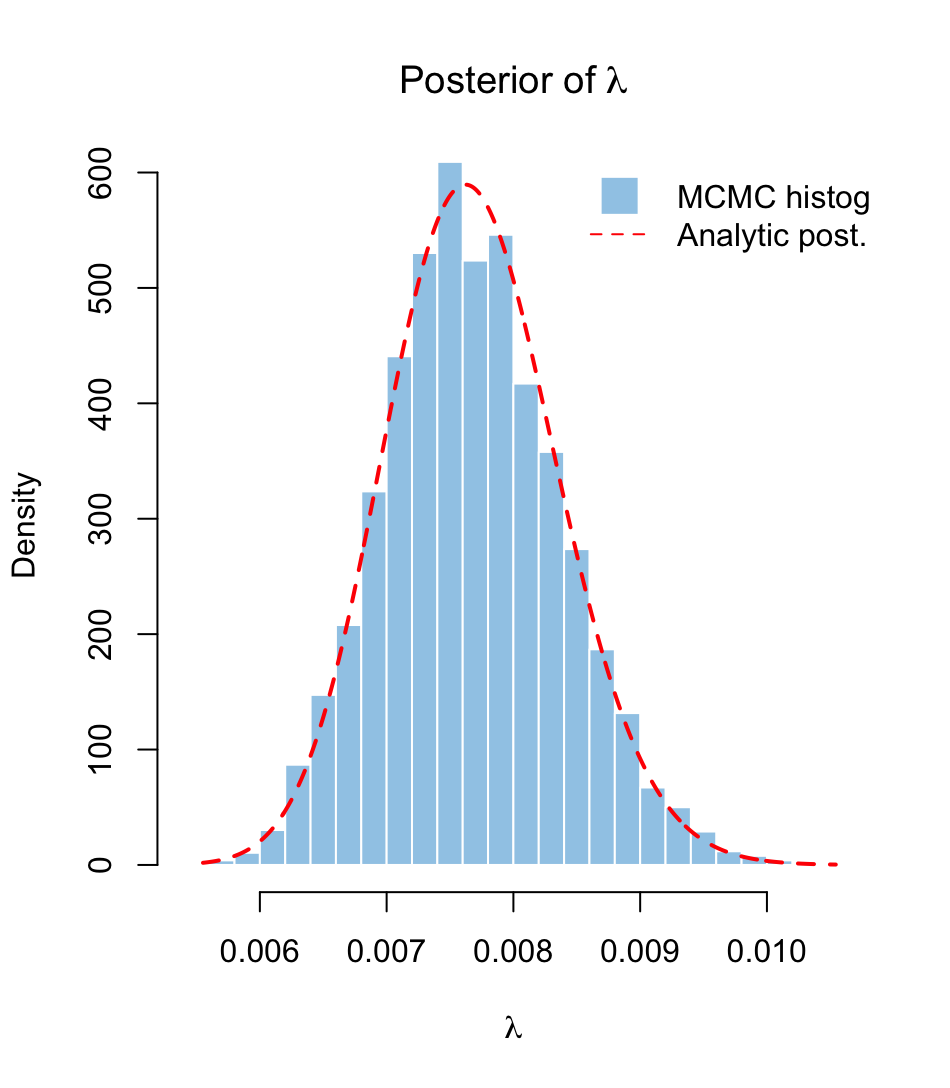
\includegraphics[height=8cm, width=0.7\textwidth]{MSc_Statistics_Research_Report_paper/images/直方图.png}
    \caption{An example posterior density}
    \label{fig:exp veteran}
\end{figure}
Posterior density plot shows the distribution and uncertainty of $\boldsymbol{\lambda}$; Trace plot shows four MCMC chains with good mixing and convergence.







%%%%%%%%%%%%%%%%%%%
%下面是指数回归模型的贝叶斯推断
%%%%%%%%%%%%%%%%%%%%%%%%%%%%%%%%%%%%%%

If introducing covariates $\mathbf{x}_i$, it is common to link the parameters and covariates through a linear regression (\cite{ibrahim2013bayesian}),
$$
\lambda_i = \exp(\mathbf{x}_i^\top \boldsymbol{\beta}),
\quad i = 1, \ldots, n,
$$
Without covariates, the hazard reduces to (\cite{chen2025survival})
$$
\lambda_i = \exp(\beta_0),
$$
representing a single baseline hazard rate for all individuals. With covariates, $\lambda_i$ varies with individual characteristics.

Here $\boldsymbol{\beta}$ are regression coefficients, and the likelihood becomes
\begin{align*}
L(D | \boldsymbol{\beta})
&= \prod_{i=1}^n 
\big[ f(y_i | \boldsymbol{\beta}) \big]^{\nu_i}
\big[ S(y_i | \boldsymbol{\beta}) \big]^{1 - \nu_i} \\
&= \prod_{i=1}^n 
\big[ \lambda_i \exp(-\lambda_i y_i) \big]^{\nu_i}
\big[ \exp(-\lambda_i y_i) \big]^{1 - \nu_i} \\
&= \prod_{i=1}^n 
\lambda_i^{\nu_i} 
\exp(-\lambda_i y_i) \\
&= \prod_{i=1}^n 
\exp\big( \nu_i \mathbf{x}_i^\top \boldsymbol{\beta} \big)
\exp\big( - y_i \exp(\mathbf{x}_i^\top \boldsymbol{\beta}) \big).
\end{align*}
In Bayesian inference, we assign priors $\pi(\theta)$, either weakly informative (e.g. $\pi(\theta)\propto1$) or informative (e.g. $\boldsymbol{\beta} \sim N(\boldsymbol{\mu}_0, \Sigma_0)$). Priors stabilize estimation, especially with small samples.

Overall, Bayesian inference proceeds by specifying the model and prior, computing the posterior
$$
\pi(\theta | D)
\propto
L(D | \theta) \times \pi(\theta),
$$
then summarizing it via means, medians, credible intervals, or posterior predictive distributions.

For example, with a normal prior, the (unnormalized) posterior is
$$
\pi(\boldsymbol{\beta} | D)
\propto
L(D | \boldsymbol{\beta})
\times
\pi(\boldsymbol{\beta}).
$$
With log posterior
$$
\log \pi(\boldsymbol{\beta} | D)
\propto \sum_{i=1}^n
\big[ \nu_i \mathbf{x}_i^\top \boldsymbol{\beta}
- y_i \exp(\mathbf{x}_i^\top \boldsymbol{\beta}) \big]
- \frac{1}{2}
(\boldsymbol{\beta} - \boldsymbol{\mu}_0)^\top
\Sigma_0^{-1}
(\boldsymbol{\beta} - \boldsymbol{\mu}_0).
$$
As this posterior lacks a closed form, MCMC methods are used for sampling (\cite{stats5010006}). Here, we implement it via \texttt{brms} in R.





%%%%%%%%%%%%%%%%%%%%%%%%%%%%
%%%%%%%%%%%%%%%%%%%%%%%%%%%%%%
%%%%%%%%%%%%%%%%%%%%%%%%%



\subsubsection{Weibull Model} \label{Weibull Model}
The Weibull model is a natural generalization of the exponential model and is suitable for describing scenarios where the hazard rate changes monotonically over time. Compared to the exponential model, which assumes a constant hazard rate, the Weibull model introduces a shape parameter $\alpha$, allowing the hazard rate $h(y)$ to increase or decrease with survival time $y$, providing greater flexibility to capture realistic survival or failure patterns.

The hazard function, probability density function, and survival function are given by:
$$
h(y) = \alpha \gamma y^{\alpha - 1}, 
\quad 
f(y) = \alpha \gamma y^{\alpha - 1} \exp(-\gamma y^{\alpha}), 
\quad 
S(y) = \exp(-\gamma y^{\alpha}),
\quad \gamma > 0,
$$
where $\alpha$ is the shape parameter and $\gamma = \exp(\lambda)$ is the scale parameter. When $\alpha > 1$, the hazard rate increases over time (indicating an aging effect); when $\alpha < 1$, the hazard rate decreases over time (indicating early failure); and when $\alpha = 1$, the Weibull model reduces to the exponential model.

Similar to the exponential case, suppose the survival time sample $Y = (Y_1, \ldots, Y_n)$ is independently and identically distributed according to a common Weibull distribution. To further incorporate individual covariate effects, the scale parameter can be modeled as:
$$
\gamma_i = \exp(\mathbf{x}_i^\top \boldsymbol{\beta}),
\quad i = 1, \ldots, n,
$$
where $\mathbf{x}_i$ denotes the covariate vector and $\boldsymbol{\beta}$ is the vector of regression coefficients. The functional forms of the hazard and density remain unchanged, with $\gamma$ replaced by $\gamma_i$.
Assuming independent samples and right-censoring, the full likelihood function is:
$$
L(\boldsymbol{\beta}, \alpha)
= \prod_{i=1}^n 
\big[ f(y_i) \big]^{\nu_i} 
\big[ S(y_i) \big]^{1 - \nu_i}
= \prod_{i=1}^n 
\big[ \alpha \gamma_i y_i^{\alpha - 1} \big]^{\nu_i} 
\exp(-\gamma_i y_i^\alpha).
$$
For the prior specification, $\boldsymbol{\beta}$ can be assigned the same normal prior as in the exponential regression case, while the shape parameter $\alpha$ is commonly assigned a Gamma prior:
$$
\boldsymbol{\beta} \sim N(\boldsymbol{\mu}_0, \Sigma_0), 
\quad 
\alpha \sim \text{Gamma}(a_0, b_0).
$$
Assuming $\boldsymbol{\beta}$ and $\alpha$ are conditionally independent a priori, the joint posterior distribution (up to a normalizing constant) is:
$$
\pi(\boldsymbol{\beta}, \alpha | D)
\propto L(\boldsymbol{\beta}, \alpha)
\, \pi(\boldsymbol{\beta})
\, \pi(\alpha).
$$
Taking logarithms yields the log-posterior kernel:
$$
\log \pi(\boldsymbol{\beta}, \alpha | D)
= \sum_{i=1}^n 
\big[
\nu_i \log \alpha + \nu_i \mathbf{x}_i^\top \boldsymbol{\beta} 
+ \nu_i (\alpha - 1) \log y_i 
- \exp(\mathbf{x}_i^\top \boldsymbol{\beta}) y_i^\alpha
\big]
+ \log \pi(\boldsymbol{\beta}) + \log \pi(\alpha) + \text{const}.
$$
As in the exponential regression case, this posterior distribution does not have a closed form and must be sampled numerically. It can be shown that, given the normal prior for $\boldsymbol{\beta}$ and Gamma prior for $\alpha$, the log-posterior is concave with respect to each parameter, satisfying the log-concavity condition and making ARS or Gibbs sampling applicable for efficient inference.

\subsubsection{Extreme Value Model}
The Extreme Value (EV) model can be viewed as a reparameterization of the Weibull model in the log-time domain, which reformulates the hazard function as an exponential-linear form in log time, facilitating direct integration of covariates.

Specifically, if the survival time $T \sim \text{Weibull}(\alpha, \gamma)$, define:
$$
Y = \log T.
$$
Then,
$$
P(Y \le y) 
= P(\log T \le y)
= P(T \le e^y)
= F_T(e^y)
= 1 - \exp\big( - \gamma e^{\alpha y} \big).
$$
Therefore, the cumulative distribution function (CDF) for the EV model is:
$$
F(y) = 1 - \exp\big( - \exp(\lambda + \alpha y) \big), 
\quad \text{where}~\lambda = \log \gamma.
$$
It follows that:
$$
\begin{aligned}
S(y) &= \exp\big( - \exp(\lambda + \alpha y) \big),\\
f(y) &= \alpha \exp(\lambda + \alpha y) \exp\big( - \exp(\lambda + \alpha y) \big),\\
h(y) &= \alpha \exp(\lambda + \alpha y).
\end{aligned}
$$
Compared to the power-form hazard in the Weibull model, the hazard in the EV model becomes exponential-linear with respect to log time and covariates, making the derivation simpler, the interpretation more straightforward, and the link with covariates naturally linear. In this formulation, $Y \in (-\infty, +\infty)$ is no longer constrained to be positive.

With covariates, the location parameter is specified as:
$$
\lambda_i = \mathbf{x}_i^\top \boldsymbol{\beta}, 
\quad i = 1, \ldots, n.
$$
Accordingly,
$$
f(y_i) = \alpha \exp(\alpha y_i + \lambda_i) \exp\big( -\exp(\alpha y_i + \lambda_i) \big), 
\quad
S(y_i) = \exp\big( -\exp(\alpha y_i + \lambda_i) \big).
$$
The observations $\{ Y_i, \nu_i \}_{i=1}^n$ are assumed to be independent and identically distributed (i.i.d.).

The likelihood function is then:
$$
L(\boldsymbol{\beta}, \alpha) 
= \prod_{i=1}^n 
\big[ f(y_i) \big]^{\nu_i} 
\big[ S(y_i) \big]^{1 - \nu_i}
= \prod_{i=1}^n 
\big[ \alpha \exp(\alpha y_i + \lambda_i) \big]^{\nu_i} 
\exp\big( -\exp(\alpha y_i + \lambda_i) \big).
$$
The prior distributions are the same as for the Weibull model:
$$
\boldsymbol{\beta} \sim N(\boldsymbol{\mu}_0, \Sigma_0), 
\quad 
\alpha \sim \text{Gamma}(a_0, b_0).
$$
The joint posterior (up to a normalizing constant) is:
$$
\pi(\boldsymbol{\beta}, \alpha | D) 
\propto L(\boldsymbol{\beta}, \alpha)
\, \pi(\boldsymbol{\beta}) 
\, \pi(\alpha).
$$
The log-kernel of the posterior is:
$$
\log \pi(\boldsymbol{\beta}, \alpha | D)
= \sum_{i=1}^n 
\big[
\nu_i \log \alpha + \nu_i \alpha y_i + \nu_i \lambda_i - \exp(\alpha y_i + \lambda_i)
\big]
+ \log \pi(\boldsymbol{\beta}) + \log \pi(\alpha) + \text{const}.
$$
It can be shown that the Hessian of this log-posterior with respect to both $\boldsymbol{\beta}$ and $\alpha$ is non-positive definite, implying log-concavity, which allows safe and efficient inference using ARS or Gibbs sampling in practice.
